\section{Introduction}
\label{sec:intro}
Knowledge graphs (KGs) represent collections of relations between real-world objects, which facilitate many downstream applications, such as semantic search~\cite{XiongPC17} and recommendation systems~\cite{ZhangYLXM2016}.
Although various KGs have been constructed in recent years, they are still highly incomplete. To be more specific, KGs built from different data sources hold unique information individually while having overlapped entities. This motivates us to integrate the knowledge of different KGs with the overlapped entities to complete KGs. 
Entity alignment (EA)~\cite{MTransE17}, a fundamental strategy for knowledge integration, has thus been widely studied. EA aims to align entities from different KGs that refer to the same real-world objects and thus facilitates the completion of KGs. 

Embedding-based EA has been proposed~\cite{MTransE17} and has been witnessed rapid development in recent years~\cite{KECG19, RREA20, AliNet20, HyperKA20, DualAMN21} thanks to the use of Graph Neural Networks (GNNs)~\cite{GCN17, GAT18, GraphSAGE17}.
They assume that the neighbors of two equivalent entities in KGs are also equivalent~\cite{AttrGNN20}. Based on this, they align entities by applying representation learning to KGs. We summarize the process of  Embedding-based EA as the following three steps: (i) taking two input KGs and collecting \emph{seed alignment} as training data; (ii) training an EA model with the isomorphic graph structure of two KGs to encode entities into embedding vectors; and (iii) aligning the equivalent entities between the two input KGs based on a specific similarity measurement (e.g., cosine similarity) of their corresponding embeddings.

% The magnitude of real-world KGs is large.
The size of real-world KGs is much larger than that of conventional datasets used in evaluating EA tasks.
% Compared with the size of the conventional datasets used in evaluating EA tasks, the scale of real-world KGs is much larger.
For instance, a real-world KG YAGO3 includes 17 million entities~\cite{LargeEA22}. Thus, EA methods should be scaled up to massive data in order to adapt to real-world applications. However, a recent proposal~\cite{LargeEA22} 
lost too much graph structure information, trading the quality of results for scalability.
% resulting in poor EA performance.
Worse still, as the input KGs becomes larger, using greedy search~\cite{OpenEA2020VLDB} to find corresponding entities \MARK{from one KG to another} with top-1-nearest neighbor becomes more challenging. 
% 
% One way to enhance the EA performance is to incorporate side information other than the graph structure of KGs. Recent methods \cite{DegreeAware20, AttrGNN20, EPEA20, EASY21, LargeEA22, CEAFF20, SEU21, BERT-INT20} propose that introducing literal information of entity names could provide a multi-aspect view for alignment models. However, compared with the methods with side information, the structure-only methods are more general~\cite{DualAMN21,RREA20, MRAEA20}. Moreover, the performances of models that incorporate machine translation on entity names are overestimated because of the name-bias issue~\cite{JEANS20, AttrGNN20, EVA20, NoMatch21}. Therefore, we should focus our attention on structure-based methods.
Specifically, the geometric properties of high-dimensional embedding vector spaces cause problems, namely, \emph{geometric problems}, for embedding-based EA, mainly including the hubness and isolation problems~\cite{OpenEA2020VLDB}.
The hubness problem indicates that some points (known as hubs) frequently appear as the top-1 nearest neighbors of many other points in the vector space.
The isolation problem implies that some outliers would be isolated from any point clusters. As the scale of input KGs grows, these problems become even more severe due to the increased number of candidates of nearest neighbor search. 

% Since most real-world entities are only represented by one entity in one KG, 
EA is generally assumed to follow 1-to-1 mapping~\cite{MTransE17}. 
% This means when aligning two KGs, for each entity in one KG, there's one, and there's only one entity in the other KG that refers to the same real-world entity.
Many existing methods have been proposed to solve the geometric problems by making the similarity matrix better satisfy this assumption, namely, \emph{normalization} methods.
% by making the similarity matrix closer to a permutation matrix.  
% We call these approaches as the \emph{normalization} process for the similarity matrix.
% \footnote{A similarity matrix may not be a square matrix. However, this kind of non-square matrix normalization could be solved easily.}.
A list of widely used normalization methods for EA is (i) \emph{Cross-domain Similarity Local Scaling (CSLS)}~\cite{CSLS} that is adopted from word translation~\cite{TransEdge19,EVA20, RREA20, EASY21}; (ii) \emph{Gale-Shapley algorithm}~\cite{GaleShapley} that treats EA as stable matching~\cite{CEAFF20,CEAFF21}; (iii) \emph{Hungarian algorithm}~\cite{Hungarian1955} and (iv) \emph{Sinkhorn iteration}~\cite{Sinkhorn13} that both transforms EA as the assignment problem~\cite{DGMC20, SEU21, EASY21}.
% In recent years, it has been pointed out that the EA task can be transformed as the assignment problem~\cite{OTEA19, DGMC20, EASY21, SEU21}. 
% The assignment problem is well-studied and can be solved using the Hungarian algorithm~\cite{Hungarian1955} or normalizing the matrix with optimal transportation~\cite{AssignProblemOT18} methods such as Sinkhorn iteration~\cite{Sinkhorn13}. 
Specifically, Sinkhorn iteration~\cite{Sinkhorn13} could significantly improve the accuracy of matching entities with embeddings~\cite{EASY21, SEU21}. Moreover, Sinkhorn iteration suits the normalization approach of EA best as it can be easily parallelized on the GPU. % which is more suitable for  Making it the most suitable normalization approach for the EA task. 
However, the existing normalization approaches~\cite{CSLS,Sinkhorn13, GaleShapley, Hungarian1955} are at least of quadratic complexity. This prohibits them from being applied to large-scale data, thus limiting their real-world applications.

In this work, we aim to scale up the normalization process of the similarity matrix to achieve higher EA performance. 
We adopt a standard machine learning technique, sampling mini-batches, to perform EA in linear time. 
Specifically, we first train a GNN model to obtain the global embeddings of two KGs.
Then, we generate mini-batches for two KGs by placing entities that could find their equivalent together. 
\MARK{Next, we calculate and normalize a local similarity matrix between two sets of entities selected for each mini-batch by Sinkhorn iteration.}
Finally, we merge these local similarities into a unified and sparse similarity matrix.
With this strategy, the final similarity matrix is normalized with Sinkhorn iteration, thus achieving higher accuracy, and the time and space complexity can also be significantly reduced. 
However, its materialization is non-trivial due to the two major challenges:
% \vspace{-5mm}
\begin{itemize}[topsep=0pt,itemsep=0pt,parsep=0pt,partopsep=0pt,leftmargin=*]
  \item \textit{How to sample mini-batches with high entity equivalence rate to ensure 1-to-1 mapping?} Splitting mini-batches on two KGs is quite different from conventional tasks. To transfer EA within mini-bathes into the assignment problem, we should place possibly equivalent entities into the same batch to meet the 1-to-1 mapping assumption. However, the mapping is only partially known (as the training set) for the EA task, making it hard for two entities to be aligned and thus to be placed in the same batch. Intuitively, randomly splitting two KGs will make most mini-batches fail to correspond. An existing study~\cite{LargeEA22} proposes a rule-based method to split batches with a higher rate of entity equivalence. However, its results are still not enough to meet the 1-to-1 mapping assumption. 
  \item \textit{How to fuse the mini-batch similarity matrices to ensure high accuracy?} The similarity matrix of each batch focuses only on its local information. Thus, the results generally deviate from those obtained without sampling, even if the batch sampler is good enough. This motivates us to study two problems. First, how to combine the similarities of these mini-batches to get a better global optimal match, after getting the mini-batch. Second, how to improve the accuracy of results obtained by batch samplers.
\end{itemize}


To tackle the above-mentioned two challenges, we propose a general EA framework, \ClusterEA{}, that can be applied to arbitrary GNN-based EA models while can be able to achieve high accuracy and scalability. 
To scale up GNN training over large-scale KGs, \ClusterEA{} first utilizes neighborhood sampling~\cite{GraphSAGE17} to train a large-scale GNN for EA in a stochastic fashion.
Then, with the embedding obtained from the GNN model, \ClusterEA{} proposes a novel \emph{strategy} for generating high-quality mini-batches in EA, namely \Sampling{}. As depicted in Figure~\ref{fig:example}, it first labels the training pairs into different batches with a \emph{clustering} method. Then it performs supervised \emph{classification} using previously labeled training pairs to generate mini-batches for all the entities. By changing the \emph{clustering} and \emph{classification} model, this strategy can sample mini-batches by capturing multiple aspects of the graph structure information. We propose two sampling methods within \Sampling{}, including
(i)  \emph{\MetisFullName{} (\MetisGCN{})} that retains the intra-KG graph structure information such as the neighborhood of nodes; and 
(ii) \emph{\KMeansFullName{} (\KMeans{})} that retains the inter-KG matching information provided by the learned embedding. 
These methods sample two KGs into multiple mini-batches with a high entity equivalent rate to satisfy the 1-to-1 mapping assumption better. 
Finally, \ClusterEA{} proposes \Merging{}, which fuses the similarity matrices calculated separately using Sinkhorn iteration with normalized global similarity. The \Merging{} process produces a matrix with high sparsity while keeping as much valuable information as possible. 
\begin{figure}[t]
% \vspace{-1mm
\centering
\hspace{-8mm}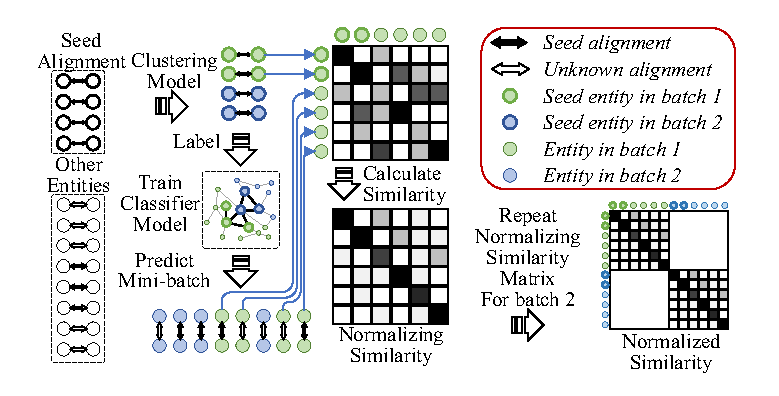
\includegraphics[width=3.55in]{figs/example.eps}
\vspace{-4mm}
\caption{An example of normalizing mini-batch similarity matrix with \Sampling{} strategy.}
\vspace{-4mm}
\label{fig:example}
\end{figure}
Our contributions are summarized as follows:

\begin{itemize}[topsep=0pt,itemsep=0pt,parsep=0pt,partopsep=0pt,leftmargin=*]
    \item{\emph{Scalable EA framework.}}
    We introduce \ClusterEA{}\footnote{Source code is publicly available at https://anonymous.4open.science/r/ClusterEA/}, a scalable framework for EA that reduces the complexity limit of normalizing similarity matrices with mini-batch. To the best of our knowledge, this is also the first framework that utilizes stochastic GNN training for large-scale EA. Any GNN model can be easily integrated into \ClusterEA{} to deal with large-scale EA (Section~\ref{sec:framework}) with better scalability and higher accuracy.
    \item{\emph{Fast and accurate batch samplers.}}
    We present \Sampling{}, a novel \emph{strategy} that sample batches by learning the latent information from embeddings of the EA model. Within the strategy, we implement two samplers to capture different aspects of KG information, including
    (i) \MetisGCN{} that focuses on retaining the intra-KG graph structure information; and
    (ii) \KMeans{} that focuses on retaining the inter-KG alignment information. Unlike the previous rule-based method, these two samplers are learning-based, thus able to be parallelized and produce high-quality mini-batches.
    \item{\emph{Fused local and global similarity matrix.}} We propose \Merging{} for normalizing and fusing not only local similarity matrices from mini-batches but also global similarity matrices into one unified sparse matrix, which enhances the expressive power of EA models. 
    \item{\emph{Extensive experiments.}} We conduct comprehensive experimental evaluation on EA tasks against state-of-the-art approaches over the existing EA benchmarks. Considerable experimental results demonstrate that  \ClusterEA{} successfully achieves satisfactory accuracy on both conventional datasets and large-scale datasets (Section~\ref{sec:exp}).
\end{itemize}

